\documentclass[12pt]{article}
\usepackage[utf8]{inputenc}
\usepackage[T1]{fontenc}
\usepackage[polish]{babel}
\usepackage{graphicx}
\usepackage{float}
\usepackage{caption}
\usepackage{subcaption}
\usepackage{amsmath}
\usepackage{hyperref}
\usepackage{geometry}
\geometry{a4paper, margin=2.5cm}

\title{Eksploracyjna analiza skupień klatek z nagrań wideo z kamer samochodowych}
\author{Dominik Banach, Marek Kacprzak}
\date{Kwiecień 2025}

\begin{document}

\maketitle

\begin{abstract}
    Celem niniejszego projektu jest eksploracyjna analiza klatek wyodrębnionych z nagrań wideo pochodzących z kamer samochodowych. Skupiono się na górnej części obrazów, zawierającej najczęściej niebo, które może pośrednio odzwierciedlać moment dnia nagrania. Obrazy zostały przekształcone z przestrzeni RGB do HSV i poddane selekcji oraz redukcji wymiarowości w oparciu o analizę zmienności pikseli. Następnie zastosowano trzy metody klastrowania: KMeans, DBSCAN i hierarchiczną metodę Warda. Najlepsze rezultaty pod względem interpretowalności uzyskano przy podziale na cztery klastry, które odpowiadają różnym warunkom widoczności – takim jak niebieskie niebo, szare niebo, noc/tunel oraz przeszkody. Dominacja klas odpowiadających szarościom może sugerować występowanie pory wieczorowej w analizowanym materiale wideo.
\end{abstract}

\section{Wstęp}
\subsection{Cel i zakres analizy}
W dobie rosnącego zainteresowania analizą danych obrazowych oraz rozwojem systemów monitoringu i autonomicznej jazdy, analiza nagrań z kamer samochodowych staje się istotnym narzędziem badawczym. Kamery montowane na pojazdach rejestrują wiele godzin materiałów wideo, które można wykorzystać do detekcji przeszkód, analizy warunków pogodowych czy oceny pory dnia. Jednym z podejść do eksploracyjnej analizy takich danych jest analiza skupień (ang. \textit{clustering}), umożliwiająca grupowanie podobnych fragmentów obrazu bez potrzeby nadzoru.

Celem niniejszego projektu jest przeprowadzenie eksploracyjnej analizy skupień na wybranym zbiorze klatek wyodrębnionych z nagrań wideo wykonanych w trakcie jazdy samochodem po Warszawie i jej obrzeżach. Skupiamy się na analizie kolorów występujących w górnej części obrazu, które często odpowiadają niebu lub wysokim zabudowaniom miejskim.

Do analizy zastosowano kilka popularnych metod klastrowania, w tym KMeans, DBSCAN oraz metodę Warda. Wcześniej konieczne było przekształcenie danych z obrazów do postaci wektorów cech, ich selekcja oraz redukcja wymiarowości. Szczególną uwagę poświęcono modelowi barw HSV, który lepiej oddaje percepcyjne różnice kolorów niż klasyczny model RGB.

Analiza pozwala odpowiedzieć na pytanie, czy na podstawie kolorystyki nieba widocznego na nagraniach możliwe jest wykrycie istotnych klas obrazów i czy dominacja poszczególnych kolorów (np. szarości) może być interpretowana w kontekście gdzie znajdował się samochód wyposażony w kamerę.

\subsection{Słownik pojęć}

\begin{itemize}
    \item \textbf{RGB (Red, Green, Blue)} – przestrzeń barw oparta na składowych światła czerwonego, zielonego i niebieskiego. Popularna w reprezentacji obrazów w kamerach i monitorach.

    \item \textbf{HSV (Hue, Saturation, Value)} – alternatywna przestrzeń barw lepiej odpowiadająca postrzeganiu kolorów przez człowieka. Składowe opisują barwę (Hue), nasycenie (Saturation) i jasność (Value).

    \item \textbf{KMeans} – popularna metoda klastrowania polegająca na podziale danych na $k$ klastrów w taki sposób, aby minimalizować odległość punktów od środków klastrów.

    \item \textbf{DBSCAN (Density-Based Spatial Clustering of Applications with Noise)} – algorytm klastrowania wykrywający gęsto zaludnione obszary w danych; nie wymaga podania liczby klastrów i radzi sobie z hałasem.

    \item \textbf{Metoda Warda} – hierarchiczna metoda klastrowania minimalizująca sumę kwadratów różnic wewnątrz klastrów. Pozwala na tworzenie dendrogramów i analizę hierarchicznej struktury danych.

    \item \textbf{Kolor nieba} – istotna cecha wizualna wykorzystywana w analizie warunków atmosferycznych. Niebieskie niebo może wskazywać na dzień, a szare na wieczór.
\end{itemize}

\section{Zbiór danych}
\subsection{Ogólny opis zbioru}

Zbiór danych wykorzystany w niniejszej analizie pochodzi z nagrań wideo zarejestrowanych za pomocą kamery samochodowej podczas przejazdu przez różne części Warszawy. Łącznie analizowany materiał obejmuje około 140 godzin jazdy, zarejestrowanych w zróżnicowanych warunkach oświetleniowych i pogodowych (np. dni pochmurne, słoneczne, zmierzch, przejazdy przez tunele lub pod estakadami).

Na potrzeby dalszej analizy z nagrań zostały wyodrębnione pojedyncze klatki (60 klatek z sekundy nagrania). Celem było uchwycenie różnorodności scen miejskich widocznych na górnej części obrazu, gdzie – zależnie od otoczenia – może występować niebo, zabudowania, infrastruktura drogowa lub bloki mieszkaniowe.

Trasa przejazdu obejmowała m.in. centrum Warszawy, mosty, dzielnice z gęstą zabudową oraz fragmenty tras szybkiego ruchu

\begin{figure}[H]
    \centering
    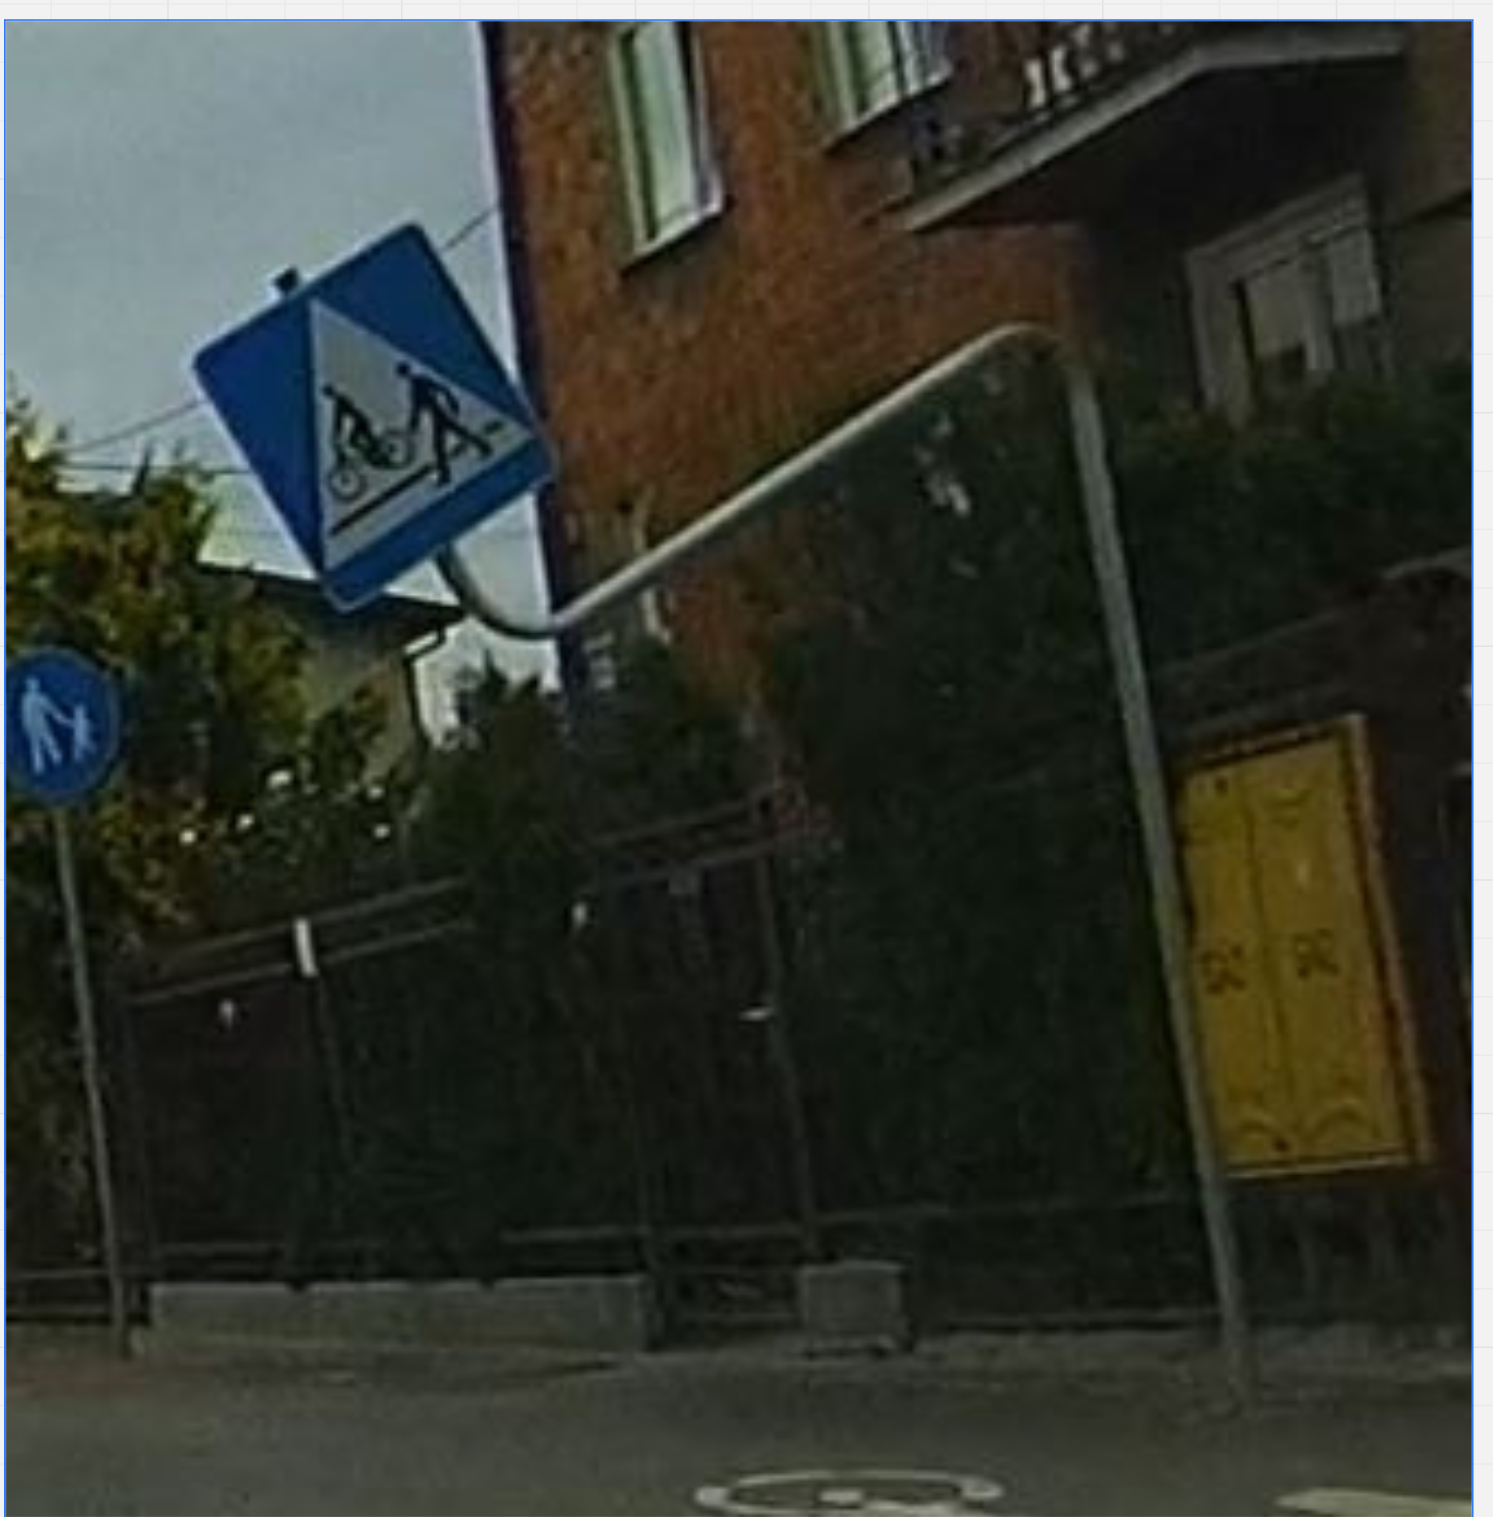
\includegraphics[width=0.8\textwidth]{mapa_trasy.png}
    \caption{Orientacyjna trasa przejazdu samochodu z kamerą.}
    \label{fig:mapa}
\end{figure}

W początkowej fazie analizy pozyskano łącznie około 60*60*140 klatek , które następnie poddano przetwarzaniu w celu dalszego modelowania i klastrowania kolorystycznego. Zastosowana metodologia koncentruje się nie na całym obrazie, lecz na jego górnej części, w której najczęściej znajduje się niebo lub elementy go przysłaniające – takie jak budynki, znaki drogowe lub elementy infrastruktury. To właśnie ta część obrazu została uznana za najbardziej reprezentatywną do klastrowania na podstawie kolorystyki sceny.

\subsection{Ekstrakcja klatek}

Z nagrań wideo pozyskanych z kamery samochodowej wyodrębniono pojedyncze klatki. Proces ekstrakcji został przeprowadzony przy użyciu skryptu automatyzującego odczyt kolejnych ramek z plików wideo oraz zapis ich jako obrazów w formacie \texttt{.png}.

Każda z klatek została przeskalowana z oryginalnej rozdzielczości $1920 \times 1080$ pikseli do mniejszej, uproszczonej postaci $240 \times 80$ piksele, co umożliwiało znaczną redukcję kosztów obliczeniowych przy dalszym przetwarzaniu. Redukcja rozdzielczości była kluczowa z uwagi na fakt, że dalsze etapy analizy wymagały konwersji każdej klatki do wektora cech.

Dla każdej przeskalowanej klatki obliczono wektor cech, w którym każdy piksel był reprezentowany trzema wartościami odpowiadającymi składowym koloru w przestrzeni RGB. Ostatecznie więc pojedynczy obraz o rozmiarze $240 \times 80$ zawierał $240 \times 80 = 19.200$ pikseli, a wektor cech miał długość $19.200 \times 3 = 57\ 600$ elementów.

Tak otrzymane wektory stanowiły bazę do dalszej redukcji wymiarowości oraz transformacji kolorystycznych, umożliwiających ekstrakcję tylko tych fragmentów obrazu, które były istotne z punktu widzenia analizy kolorystyki nieba lub jego braku.

\subsection{Dalsza redukcja wymiarowości}

\subsubsection{Analiza średniej klatki}

Pierwszym krokiem redukcji danych było obliczenie tzw. średniej klatki, czyli uśrednienia wartości pikseli dla wszystkich wyodrębnionych obrazów. Celem tego zabiegu była identyfikacja wspólnych, statycznych elementów występujących w większości klatek, które nie niosą dodatkowej informacji istotnej dla klastrowania.

W wyniku analizy zaobserwowano wyraźną obecność odbić deski rozdzielczej oraz maski samochodu w dolnej części obrazów. Te elementy występowały regularnie i stanowiły silnie powtarzalny wzorzec, który mógłby zdominować dalszą analizę skupień. Na podstawie obserwacji średniej klatki zdecydowano się na obcięcie dolnych 20 wierszy obrazu, co odpowiadało około jednej trzeciej jego wysokości.

Tym samym analizowany fragment każdej klatki został ograniczony do wymiaru $240 \times 60$ piksele, co odpowiadało nowemu wektorowi cech o długości $240 \cdot 60 \cdot 3 = 43\ 200$ elementów w przestrzeni RGB.

\begin{figure}[H]
    \centering
    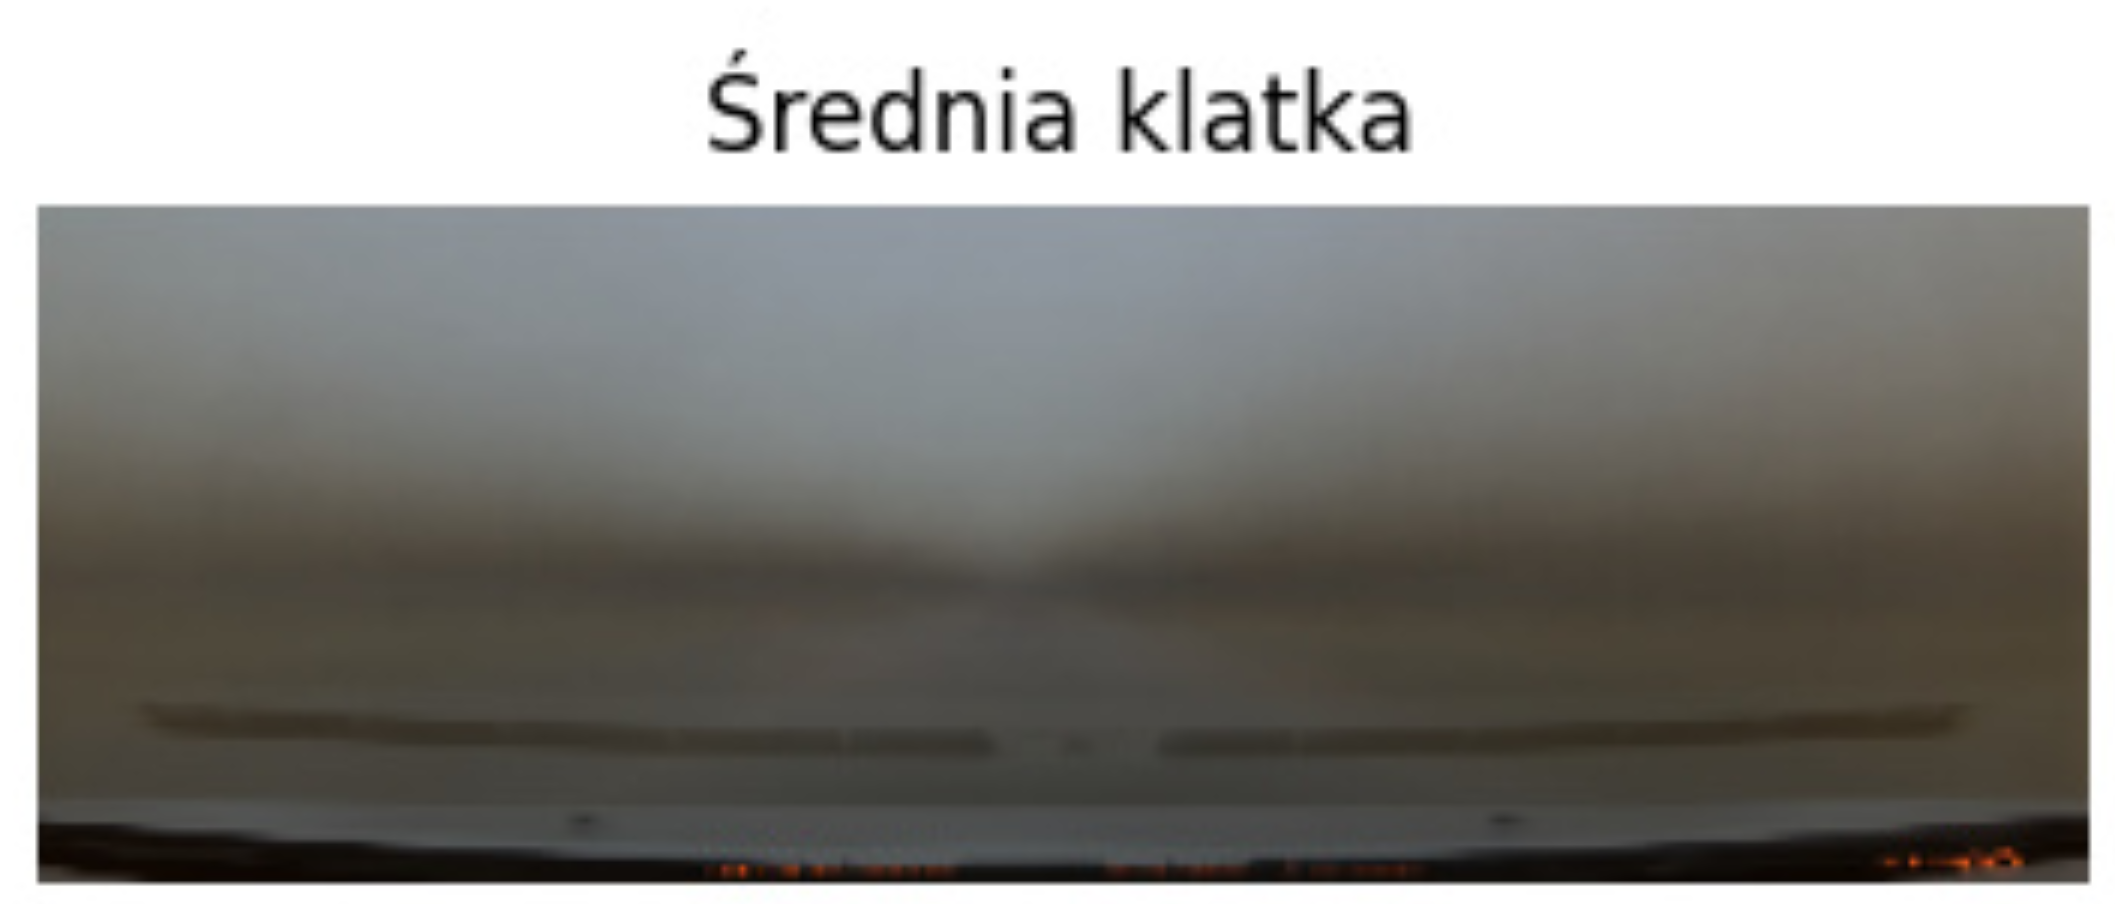
\includegraphics[width=0.6\textwidth]{średnia_klatka.png}
    \caption{Obraz średniej klatki – widoczne powtarzalne elementy w dolnej części (maska, deska rozdzielcza).}
    \label{fig:srednia_klatka}
\end{figure}

\subsubsection{Analiza współczynnika zmienności (CV)}
Analiza współczynnika zmienności pikseli, wybór obszarów z CV $\leq$ 20\%, które odpowiadają niebu.

\subsubsection{Konwersja na model HSV i statystyki opisowe}
Opis konwersji z RGB na HSV, przedstawienie statystyk opisowych zredukowanego zbioru, wizualizacje 2D i 3D.

\subsubsection{Propozycja dwóch ostatecznych wektorów cech}
Opis dwóch wybranych wektorów cech, które najlepiej sprawdziły się w analizie.

\section{Klastrowanie KMeans}
\subsection{Krótszy wektor cech}
Wykres łokciowy, wizualizacje 3D klastrów, przykładowe obrazy z klastrów.

\subsection{Dłuższy wektor cech}
Brak wykresu łokciowego, wizualizacje klastrów, przykładowe obrazy z klastrów.

\subsection{Interpretacja wyników}
Interpretacja czterech klastrów: niebieskie niebo, szare niebo, noc/tunel, przeszkody.

\section{Klastrowanie DBSCAN}
\subsection{Wybór parametru eps}
Wykres 5NN do wyboru parametru eps.

\subsection{Wizualizacje dla różnych wartości MinPts}
Wizualizacje klastrowania dla eps=0.008 i różnych wartości MinPts, analiza wyników.

\subsection{Porównanie z KMeans}
Porównanie podziału na 4 klastry DBSCAN i KMeans, trudności w interpretacji klastrów DBSCAN.

\section{Klastrowanie metodą Warda}
\subsection{Dendrogram}
Prezentacja dendrogramu uzyskanego metodą Warda.

\subsection{Podziały na 3, 4 i 5 klastrów}
Wizualizacje podziałów na różną liczbę klastrów, analiza podobieństw do wyników KMeans.

\subsection{Interpretacja i porównanie z KMeans}
Interpretacja klastrów uzyskanych metodą Warda, porównanie z wynikami KMeans.

\section{Wnioski}
Podsumowanie wyników analizy, dominacja szarego nieba, stosunek niebieskiego do szarego nieba, odniesienie do pracy z konferencji EPEC 2024 dotyczącej wpływu zanieczyszczeń na kolor nieba.

\begin{thebibliography}{9}
    \bibitem{epec2024}
\end{thebibliography}

\end{document}
